%%%%%%%%%%%%%%%%%%%%%%%%%%%%%%%%%%%%%%%%%
% Beamer Presentation
% LaTeX Template
% Version 1.0 (10/11/12)
%
% This template has been downloaded from:
% http://www.LaTeXTemplates.com
%
% License:
% CC BY-NC-SA 3.0 (http://creativecommons.org/licenses/by-nc-sa/3.0/)
%
%%%%%%%%%%%%%%%%%%%%%%%%%%%%%%%%%%%%%%%%%

%----------------------------------------------------------------------------------------
%	PACKAGES AND THEMES
%----------------------------------------------------------------------------------------

\documentclass[14pt,aspectratio=169]{beamer}

\mode<presentation> {


% The Beamer class comes with a number of default slide themes
% which change the colors and layouts of slides. Below this is a list
% of all the themes, uncomment each in turn to see what they look like.

% \usetheme{default}
% \usetheme{AnnArbor}
% \usetheme{Antibes}
% \usetheme{Bergen}
% \usetheme{Berkeley}
% \usetheme{Berlin}
% \usetheme{Boadilla}
% \usetheme{CambridgeUS}
% \usetheme{Copenhagen}
% \usetheme{Darmstadt}
% \usetheme{Dresden}
% \usetheme{Frankfurt}
% \usetheme{Goettingen}
% \usetheme{Hannover}
% \usetheme{Ilmenau}
% \usetheme{JuanLesPins}
% \usetheme{Luebeck}
% \usetheme{Madrid}
% \usetheme{Malmoe}
% \usetheme{Marburg}
% \usetheme{Montpellier}
% \usetheme{PaloAlto}
% \usetheme{Pittsburgh}
% \usetheme{Rochester}
% \usetheme{Singapore}
% \usetheme{Szeged}
% \usetheme{Warsaw}

% \setbeamercolor*{frametitle}{parent=palette primary}
% \setbeamerfont{block title}{size={}}

\setbeamertemplate{frametitle}{
    \vspace{1em}
    \textbf{\insertframetitle}
}

% As well as themes, the Beamer class has a number of color themes
% for any slide theme. Uncomment each of these in turn to see how it
% changes the colors of your current slide theme.

% \usecolortheme{albatross}
% \usecolortheme{beaver}
% \usecolortheme{beetle}
\usecolortheme{crane}
% \usecolortheme{dolphin}
% \usecolortheme{dove}
% \usecolortheme{fly}
% \usecolortheme{lily}
% \usecolortheme{orchid}
% \usecolortheme{rose}
% \usecolortheme{seagull}
% \usecolortheme{seahorse}
% \usecolortheme{whale}
% \usecolortheme{wolverine}

%\setbeamertemplate{footline} % To remove the footer line in all slides uncomment this line
%\setbeamertemplate{footline}[page number] % To replace the footer line in all slides with a simple slide count uncomment this line

%\setbeamertemplate{navigation symbols}{} % To remove the navigation symbols from the bottom of all slides uncomment this line
}

\definecolor{darkblue}{RGB}{32, 43, 56}
\definecolor{lightblue}{RGB}{203, 220, 239}
\definecolor{red}{RGB}{201, 42, 42}
\setbeamercolor*{palette primary}{bg=darkblue,fg=white}
\setbeamercolor*{palette quaternary}{bg=lightblue}
\setbeamercolor{section in toc}{fg=darkblue,bg=white}
\setbeamercolor{title}{fg=white,bg=darkblue}

% \setbeamercolor{background canvas}{bg=black}
% \setbeamercolor{normal text}{fg=white}

\usepackage{graphicx} % Allows including images
\usepackage{booktabs} % Allows the use of \toprule, \midrule and \bottomrule in tables
\usepackage{hyperref}
\usepackage{minted}
\renewcommand{\MintedPygmentize}{./pygmentize.py}

\usepackage{amssymb}
\usepackage{pifont} % for checkmarks
\newcommand{\cmark}{\ding{51}}%
\newcommand{\xmark}{\ding{55}}%

% fonts
\usepackage[T1]{fontenc}
\usepackage[extrabold]{inter}
\usefonttheme[onlymath]{serif}
\usefonttheme{structurebold} 

% frame breaks don't add numbers to slide title
\setbeamertemplate{frametitle continuation}{}

% large split between lines
\setlength{\parskip}{\baselineskip}

\newenvironment{slide}[1]
    {\begin{frame}[containsverbatim,allowframebreaks,noframenumbering]
        \frametitle{#1}
    }
    {\end{frame}}

\newenvironment{slidefull}
    {
        \setbeamercolor{background canvas}{bg=darkblue}
        \setbeamercolor{normal text}{fg=white}
        \usebeamercolor[fg]{normal text}
        \begin{frame}
    }
    {\end{frame}}


%----------------------------------------------------------------------------------------
%	TITLE PAGE
%----------------------------------------------------------------------------------------


\title{PRQL}
\subtitle{Pipelined Relational Query Language}

\titlegraphic{\vspace*{-2em} \includegraphics[height=4em]{./images/prql-logo.pdf}}
% \logo{\includegraphics[width=2em]{./images/prql-logo.pdf}}

\author{\large Aljaž Mur Eržen}

\institute{\small Compiler developer @EdgeDB}

\date{}

\begin{document}

\begin{frame}
\titlepage

% I'm aljaz mur erzen, I work at EdgeDB as a compiler engineer and today I'll talk about prequel.
% Prequel is a new language that was born out of frustrations with SQL and dataframe libraries.

\end{frame}

\begin{slide}{}

% Before I get started, I'll briefly show you how does it look like, so you have a mental image of what we are dealing with.

\begin{minted}{PRQL}
from albums
filter album_id > 100
sort albums.title
take 10
join artists (==artist_id)
select {
    albums.album_id,
    albums.title,
    f"Artist name: {artist.name}",
}
\end{minted}

% This query is meant to execute in a database that contains tables `albums` and `artists`.
% <!-- explanation of what the query does -->

% Cool. It looks similar to SQL and (also Python is some cases).
% I do think that just by looking at this example you should be able to write simple queries yourself.

\end{slide}


\begin{slide}{}
\Large
% But any time that I'm presented with a new language, my first question is "Why?".
% Why dear god do we need more strange syntax, more new rules and more slightly different function names than what I'm already used to?   

Why?

% And this is a very relevant question, because any new tool (and even more so a language) has a significant transition cost associated with it.

There are transition costs!

% So that is the main question I'll be answering today, and this is going to take some time.
% From time to time it might seem like I'm bashing SQL for the fun of it, and this is partially true.
% It also partially because PRQL was designed out of contempt toward data tools we were dealing with.

\end{slide}
    


\begin{frame}
\frametitle{Overview}
\tableofcontents

% A few notes:
% - when I say "a database", I mean "a database management system" (mostly relational)

\end{frame}

\section{Flaws of SQL}

\begin{slidefull}
\Large A deef dive into

\LARGE \textbf{Flaws of SQL}
\end{slidefull}


\begin{slide}{Origins of the relational model}

% The relational model was introduced by Edgar F. Codd in a 1970 paper “A Relational Model of Data for Large Shared Data Banks”.

% The proposed novelty was abstraction over data storage, so a user of "data banks" did not have to deal with where and how the data is stored, but work with data in its relational form.

1970, Edgar F. Codd: abstraction over data storage

$\rightarrow$ Tuple relational calculus

% Soon after, people figured out that "tuple relational calculus" is not the most readable to regular users as it was expressed with greek letters and Donald D. Chamberlin and Raymond F. Boyce published a paper that introduced SEQUEL: A structured English query language.
    
% It was presented as having the same expressive power as the first order predicate calculus, on which the tuple relational calculus was based on. It was meant for "users without formal training in mathematics or computer programming" and "predominant use of the language would be for ad-hoc queries".

1974, Donald D. Chamberlin \& Raymond F. Boyce: SEQUEL

$\rightarrow$ Not a ``proper'' programming language

% As in - SQL was not meant to be a "proper" programming language.

\end{slide}


\begin{slide}{Not really composable}

\begin{minted}{SQL}
SELECT album_id, COUNT(*) AS track_count
FROM tracks GROUP BY album_id
\end{minted}

\framebreak

\begin{minted}{SQL}
SELECT i.album_id, i.track_count, a.artist_id
FROM (
  SELECT album_id, COUNT(*) AS track_count
  FROM tracks GROUP BY album_id
) AS i
JOIN albums a USING (album_id)
\end{minted}
\end{slide}


\begin{slide}{Patched syntax}

\begin{minted}{SQL}
SELECT
  SUM(total)
FROM
  invoices
\end{minted}

\framebreak

\begin{minted}{SQL}
SELECT
  total / SUM(total) OVER () AS normalized_total
FROM
  invoices
\end{minted}

\framebreak

\begin{minted}{SQL}
SELECT DISTINCT name
FROM invoices
\end{minted}

\framebreak

% If you look at this SWITCH statement, you will be
% so taken back by its verbosity and screaming uppercase,
% that you will not notice that it is actually COBOL 

\begin{minted}{SQL}
SELECT EVALUATE TYPE-EMPLOYEE
  WHEN "F" 
    MOVE "FULL TIME" TO EMP-TYPE-PR
  WHEN "P" 
    MOVE "PART TIME" TO EMP-TYPE-PR
  WHEN "C" 
    MOVE "CONSULTANT" TO EMP-TYPE-PR
  WHEN OTHER
    MOVE "INVALID" TO EMP-TYPE-PR
\end{minted}

% And that's my point: SQL is old and lacking modern
% language features such a f-strings and trailing commas.

% And we cannot add them in, because they would break
% existing parsing rules.

Too much syntax

... but also ...

Not enough syntax

\end{slide}


\begin{slide}{Name resolution}

\begin{minted}{SQL}
SELECT title AS title_alias
FROM albums
\end{minted}

\framebreak

% clause    title   title_alias
% WHERE     x       
% GROUP BY  x       x
% ORDER BY  x       x
% HAVING    x

\begin{minted}{SQL}
SELECT title AS title_alias
FROM albums
WHERE title_alias LIKE 'Do I Wanna %'
GROUP BY title_alias
ORDER BY title_alias
\end{minted}

\framebreak

More rules:

-- ORDER BY positionals

-- Correlated subqueries

-- LATERAL

\end{slide}


\begin{slide}{Relations vs scalars}

% SQL has two major categories of expressions:
% relational and scalar

% Both can be returned from a SELECT statement

% Here, first returns a relation, second returns a scalar

\begin{minted}{SQL}
SELECT * FROM table

SELECT count(*) FROM table
\end{minted}

\framebreak

% They have the same syntactical structure
% They cannot be used in all the same places

\begin{minted}{SQL}
SELECT emp_id FROM emp WHERE role = 'manager'
\end{minted}

\framebreak

\begin{minted}{SQL}
SELECT *
FROM emp
WHERE emp_id = (
    SELECT emp_id FROM emp WHERE role = 'manager'
)
\end{minted}

\end{slide}

\begin{slide}{Relations cannot be ordered}

\begin{minted}{SQL}
SELECT * FROM albums ORDER BY title
\end{minted}

\framebreak

\begin{minted}{SQL}
SELECT
  *,
  ... AS my_col
FROM (
    SELECT * FROM albums ORDER BY title
) inner
\end{minted}

\framebreak

\begin{minted}{SQL}
SELECT
  *,
  ROW_NUMBER()
    OVER (ORDER BY artist_id) AS my_col
FROM (
    SELECT * FROM albums ORDER BY title
) inner
\end{minted}

\framebreak

SELECT returns an \textbf{ordered set}

FROM pulls-in a \textbf{set}
\framebreak

\begin{minted}{SQL}
SELECT
  *,
  ... AS my_col
FROM (
    SELECT *
    FROM albums
) inner
ORDER BY title
\end{minted}

\begin{minted}{SQL}
SELECT
  *,
  ... AS my_col
FROM (
    SELECT * FROM albums ORDER BY title LIMIT 10
) inner
ORDER BY title
\end{minted}

\end{slide}

\begin{slide}{Identity of aggregation}

\begin{minted}{SQL}
SELECT SUM(cost) FROM expenses WHERE FALSE
\end{minted}

Two possible behaviors: NULL or 0

Both valid

\framebreak

\begin{block}{}
    \textbf{``Every marble in this bag is black''}

    ... but the bag is empty.
\end{block}

Ancient greeks say FALSE

Modern logic says TRUE

SQL says NULL

% \framebreak

% This breaks stuff

% \begin{minted}{SQL}
% SELECT array_agg(value)
% FROM jsonb_array_elements(my_jsonb_array)
% \end{minted}

\framebreak

\textbf{Homomorphism of addition}

\begin{verbatim}
SUM([1]) + SUM([4, 5]) = SUM([1, 4, 5])

                 1 + 9 = 10 
\end{verbatim}

\framebreak

\begin{verbatim}
SUM([1]) + SUM([]) = SUM([1])

       1 +    ?    = 1

        -> SUM([]) = 0
\end{verbatim}

\textbf{identity of addition}

\framebreak

\large
\begin{verbatim}
COUNT([])      = 0
ARRAY_AGG([])  = []
SUM([])        = 0
ANY([])        = false
EVERY([])      = true
STRING_AGG([]) = ''
\end{verbatim}

\end{slide}


\begin{slide}{Dialects}


    % There is a lot of databases and each of them supports different language features.

    % Most differences are on the syntactic level (TOP vs LIMIT, or DISTINCT ON).

Differences in:

- syntax (TOP vs LIMIT)

    % There are differences in what functions are available.
    
- available functions

    % There are differences in what data types are available (datetime in SQLite, arrays in MySQL).

- available data types

\framebreak

% So there is no SQL language, just a class of languages that look similar.

A class of languages

There is a standard

Slight deviations
    
\framebreak

% ... and actually, we could expect this. Each database has different:
% - priorities on what's important,
% - backward compatibility guarantees (you cannot just change behavior for the sake of standard conformity),
% - limitations of what it is possible to implement with current architecture.

Different:

- priorities

- backward compatibility guarantees

- implementation limitations

\framebreak

% The problematic part is that the database interface does not exactly specify what it supports.
% There is documentation, but man, imagine if you have a large query and your boss asks you
% "can we execute this on some other database engine?".
% Best you can say is "probably".

% We lack a specification of all supported features of a database engine.

No clear \& robust specification

Compilers could:

- adapt query to target database

- produce error early

% Something that you can run your compiler against, and would:
% - produce a slightly different query to be executed, but with same behavior,
% - produce errors like
%   "this function is not supported by your database, use that function instead".

% I'll talk about how we tackle this problem and out long-term plan.

\end{slide}


\section{Language for relations}
\begin{slidefull}
\Large Design of a new

\LARGE \textbf{Language for relations}
\end{slidefull}


\begin{slide}{Tuple relational calculus}

% In short, this is relational algebra:

Relation $\sim$ a set of tuples

\vspace{2em}

\Large

$\pi_{track\_id, name, title}(R)$

$\sigma_{track\_id = 5}(R)$

$R * S$

% I'll go over fundamentals of PRQL syntax and semantics.
% I want to show that if you go and design a language that is able to express relational algebra,
% - using modern understanding of type systems,
% - aim for it to be minimal and ergonomic,
% - using syntax similar to other popular languages right now
% ... you will end up with the design of PRQL (or something very similar).

% In other words, the design decisions we took are obvious choices within our requirements.   

\end{slide}

\begin{slide}{Data model}

{\Large Basic data types}

\vspace{-1em}
\begin{verbatim}
bool, int, float, str
\end{verbatim}
\vspace{-1em}

\framebreak


{\Large Tuples}

\vspace{-1em}
\begin{verbatim}{my_int = 5, 4.2, my_bool = true}\end{verbatim}
\vspace{-1em}

\begin{itemize}
\item named fields
\item different types
\item static number of fields
\end{itemize}

\framebreak


{\Large Arrays}

\vspace{-1em}
\begin{verbatim}[1, 2, 10, -3]\end{verbatim}
\vspace{-1em}

\begin{itemize}
\item unnamed items
\item items have the same type
\item dynamic number of items
\end{itemize}


\framebreak


Relations $\sim$ an array of tuples 

\begin{minted}{PRQL}
[
    {my_int =  5, 4.2, my_bool = true},
    {my_int = -2, 6.1, my_bool = false},
    {my_int = 12, 3.0, my_bool = false},
]
\end{minted}

% Not exactly the same as relational model.
% - arrays are ordered,
% - tuple fields can be unnamed,

\end{slide}

\begin{slide}{Declarations}
\Large
\begin{minted}{PRQL}
let a = 5

let b = a + 1
\end{minted}

\end{slide}

\begin{slide}{Functions}
\Large
\begin{minted}{PRQL}
let add_one = x -> x + 1

let add = x y -> x + y
\end{minted}

\framebreak

\begin{minted}{PRQL}
let five = (add_one 4)

let six = (add 4 2)
\end{minted}

\framebreak

\begin{minted}{PRQL}
let seven = (5 | add_one | add_one)

let seven = (
    5
    add_one
    add_one
)
\end{minted}
\vspace*{-2em}

\end{slide}

\begin{slide}{Transforms}
\large
% Ok, so know how functions behave and how they can be used.
% I'll now show how we can use this same function semantics to operate on relations.
% Functions that operate on relations are called transforms. 

% Let's say that there is a variable invoices, which is a relation, doesn't where it's data comes from.
% Now we can define a variable res, which will call function filter,
% applied to a row expression and the invoices relation.

\begin{minted}{PRQL}
let invoices = ...

let main = (filter (total > 10) invoices)
\end{minted}

% Now let's simplify this notation a bit.
% First, let's use pipeline notation for filter

\framebreak
\begin{minted}{PRQL}
let invoices = ...

let main = (invoices | filter (total > 10))
\end{minted}

% Actually, the longer one 

\framebreak
\begin{minted}{PRQL}
let invoices = ...

let main = (
    invoices
    filter (total > 10)
)
\end{minted}

% If you look at the `res` variable - that is the main var that we want to return from the query.
% PRQL has a rule that if such variables are last declarations in a query,
% they can omit the `let main` and be just plain expressions

\framebreak
\begin{minted}{PRQL}
let invoices = ...

invoices
filter (total > 10)
\end{minted}

% Because our `invoices` relation is actually stored in database table,
% we can use `from` function, which will pull the relation from the database.

\framebreak
\begin{minted}{PRQL}
from invoices
filter (total > 10)
\end{minted}

% As the last touch, the parenthesis are not really needed.

\framebreak
\begin{minted}{PRQL}
from invoices
filter total > 10
\end{minted}

% And this is an idiomatic PRQL query.
% Built on a few basic syntactic and semantic rules.
% With formal specification that would probably fit on a few pages.

\end{slide}

\begin{slide}{Top to bottom}

\begin{minted}{PRQL}
from albums
filter album_id > 100
sort albums.title
\end{minted}

\framebreak

\begin{minted}{PRQL}
from albums
filter album_id > 100
sort albums.title
take 10
\end{minted}

\framebreak

\begin{minted}{PRQL}
from albums
filter album_id > 100
sort albums.title
take 10
join artists (==artist_id)
\end{minted}

\framebreak

\begin{minted}{PRQL}
from albums
filter album_id > 100
sort albums.title
take 10
join artists (albums.artist_id == artists.artist_id)
\end{minted}

\framebreak

\begin{minted}{PRQL}
from albums
filter album_id > 100
sort albums.title
take 10
join artists (==artist_id)
select {
    albums.album_id,
    albums.title,
    f"Artist name: {artist.name}",
}
\end{minted}

\framebreak

- Convenient for exploration

- Lazy evaluation

- Extract a variable

- Extract a function

\framebreak

\begin{minted}{PRQL}
let take_cheapest = n rel -> (
    rel
    sort unit_price
    take n
)

from tracks
take_cheapest 5
\end{minted}

\end{slide}


\begin{slide}{Orthogonal}

\begin{minted}{PRQL}
from expenses
filter dept == "Sales"
aggregate {total = sum cost}
filter total > 100.00
\end{minted}

\large
\texttt{WHERE} $\mapsto$ \texttt{filter}
\hfill
\texttt{HAVING} $\mapsto$ \texttt{filter}

\framebreak

% There is an important aspect to PRQL's design, which we call
% transform orthogonality. It means that transforms (functions on relations)
% should do one thing, and do it well. Here this would mean that transforms
% have invariants - contract that says a property of the relation will not be changed.

Transform invariants:

- \texttt{filter} will not change columns

- \texttt{derive} \& \texttt{select} will not change number of rows

% this is not true for SQL clauses: SELECT may also imply aggregation

- \texttt{aggregate} will produce exactly one row

% This invariants make transforms compose nicely and it keeps the number of transforms low.

% A great example of this is aggregate:
\end{slide}

\begin{slide}{Grouping}

\begin{minted}{PRQL}
from expenses
aggregate {total = sum cost}


[
    {total = 431.22},
]
\end{minted}

% aggregate is a transform
% sum is an aggregation function
% total is the sum of column cost

\framebreak

% let's say we want expenses by each value in dept_no column

% we partition the relation by values of dept_no column
% we apply the aggregate function to each of the partitions
% we combine the partitions back together, prefixing with dept_no column

\begin{minted}{PRQL}
from expenses
group dept (
    aggregate {total = sum cost}    
)

[
  {dept = "Sales",      total = 331.00},
  {dept = "Accounting", total = 100.22},
]
\end{minted}

\framebreak

\begin{minted}{PRQL}
from expenses
group dept (
    take 1    
)

[
  {dept = "Sales",      id = 33, cost =  5.30},
  {dept = "Accounting", id = 45, cost = 12.22},
]
\end{minted}

\framebreak

\begin{minted}{PRQL}
from expenses
group dept (
    sort {-cost}
    take 1
)

[
  {dept = "Sales",      id = 33, cost = 5.30},
  {dept = "Accounting", id = 16, cost = 1.22},
]
\end{minted}

\framebreak

\large
\begin{minted}{PRQL}
from expenses
group expenses.* (
    take 1
)
\end{minted}

\framebreak

\large
\begin{minted}{PRQL}
from expenses
group expenses.* (
    take 1
)
\end{minted}

\begin{minted}{SQL}
SELECT DISTINCT *
FROM expenses
\end{minted}

\end{slide}

\begin{slide}{Nulls}

% This was all "big picture" stuff - fundamentals of PRQL design
% They provide a shift in thinking when working with relations.

% Now it's time to talk about little things that make PRQL ergonomic.

% If you know about SQL behavior, you know it makes sense on some level,
% but you also know that it is inconvenient.

% In PRQL, null is a value.

\large

\begin{minted}{PRQL}
# PRQL
null == null  # true

my_col == null
\end{minted}

\begin{minted}{SQL}
-- SQL
my_col IS NULL
\end{minted}

\end{slide}

\begin{slide}{Micro-features}

\begin{minted}{PRQL}
from employees
derive {
  age = @2023-01-31 - birth_date,
  full_name = f"{first_name} {last_name}",
  manager = reports_to ?? "No one",
#  is_fired = "No",
  salary = 1_000_000,
}
\end{minted}

\end{slide}

\section{Compiling queries}
\begin{slidefull}
\Large Challenges of

\LARGE \textbf{Compiling queries}
\end{slidefull}

%%% --- omitted ---
%%% Integrating a language into a database comes with a few downsides.
%%% 
%%% If you reuse some existing language (like SQL):
%%% - you have to implement it with all of its quirks that people are already used to,
%%% - you will certainly diviate from the language at some point,
%%% 
%%% If you create a new language:
%%% - you have to design a language alogside an already complex system,
%%% - it will lack a few features,
%%% - people will have to learn it,


\begin{slide}{SQL as a compilation target}

\large

% Now I need to talk about the elephant in the room. How is this new language executed?

How is this language executed?

% Short answer: we have a compiler to SQL

% As I've said, it is meant to replace SQL, but this is only partially true.
% SQL is two things:
% - a database interface
% - a language for querying 

\xmark \hspace{0.5em} database interface

% well it could, but still not all SQL statements (REINDEX, CREATE, ...)
% every database would have to add support for it

% What I mean, is that it replaces the language that people use to express their data transformations.

\cmark \hspace{0.4em} a query language

% What is a query language, why do we even need it?

\end{slide}


\begin{slide}{The task of a query lanuage}

Imagine a database without a query language.

% Well, you'd need some kind of interface, so imagine there is an API where you specify a table that you want to query.

% That would be equivalent to issuing `SELECT * FROM albums`

\begin{minted}{SQL}
SELECT * FROM albums
\end{minted}

% and then filter and join in your super fast Rust code.

... and then transform in client code.

% That would be super slow, as it would transfer way too much data to the client, just to be thrown away later.

$\rightarrow$ super slow

% To be fair, we could also include the `WHERE` clause in our API, but that still doesn't solve all the problems.

\framebreak

% A more extreme example is this,
% where we do some processing on our data and return a single number.

Extreme example:

\begin{minted}{SQL}
SELECT COUNT(*)
FROM albums
WHERE title LIKE 'The %'
\end{minted}

\framebreak

% What you want is for this processing to happen as close to the data as possible.

\textbf{Processing should be close to data}

% This is the ideal scenario because:

- minimal data transfer

% this is obvious, if we don't transfer data from the database to the client there is less things to do.
%  and as the saying goes, best way to make a program faster is to do less.

- parallelism
% your database might be enormous, spanned over multiple nodes.
% this is possible to achieve with general programming languages,
% but it is not easy.

- vectorization
% some operations (eg. a sum of two columns) can be compiled to vectorized CPU instructions.
% this gives enormous performance boost (see DuckDB or Polars)

%%% --- omitted ---
%%% As people who worked with MapReduce know, this query is embarrassingly simple to parallelize.

\framebreak

% So essentially, we are giving the database a program that we want executed and the database does that for you, before returning the data.

% Which makes the database an execution platform or a compilation target.

Databases are:

- execution platforms

- compilation targets

Analogous to amd64, JVM

% Similarly as when:
% - a Rust program compiles to a binary to be executed on a amd64 processor, for example, and
% - a Java program compiles to byte code to be executed in JVM,
% - -> we compile PRQL to SQL to be executed in a database.

\end{slide}


\begin{slide}{Leaky abstractions}

% We want the database interface to be transparent to the user.

Database interface should be transparent

Currently, this is not the case:

- invalid SQL

- sub-optimal SQL

- runtime errors

\end{slide}

%%% -- omitted --
%%% \begin{slide}{A better database interface}
%%% When an SQL query is received by a database, it hits another compiler. It is parsed, de-sugared, resolved and compiled into a query plan - an object the database can then execute.
%%% 
%%% So when we started thinking about SQL as a compilation target, we saw a few things that could be improved, if we were replace the SQL with a more rigid query representation.
%%% 
%%% Because the interaction with the database happens at runtime, we would want to:
%%% - minimize runtime query processing (to improve performance and simplify tooling),
%%% - remove ambiguity,
%%% - easy to extend,
%%% 
%%% substrait.io
%%% \end{slide}


\section{PRQL, the project}
\begin{slidefull}
\LARGE \textbf{PRQL, the project}

\Large -- an opensource effort
\end{slidefull}

% 2022: PRQL started as a proposal for a new database query language
% 

\begin{slide}{The compiler and its IRs}

prqlc: compiler from PRQL to SQL

targets: sql.postgres, sql.sqlite, sql.duckdb, sql.mysql, sql.clickhouse

bindings for C, Python, JS, Java, .NET, PHP

\framebreak

Don't connect, infer

Fail early

\vspace*{-0.5em}
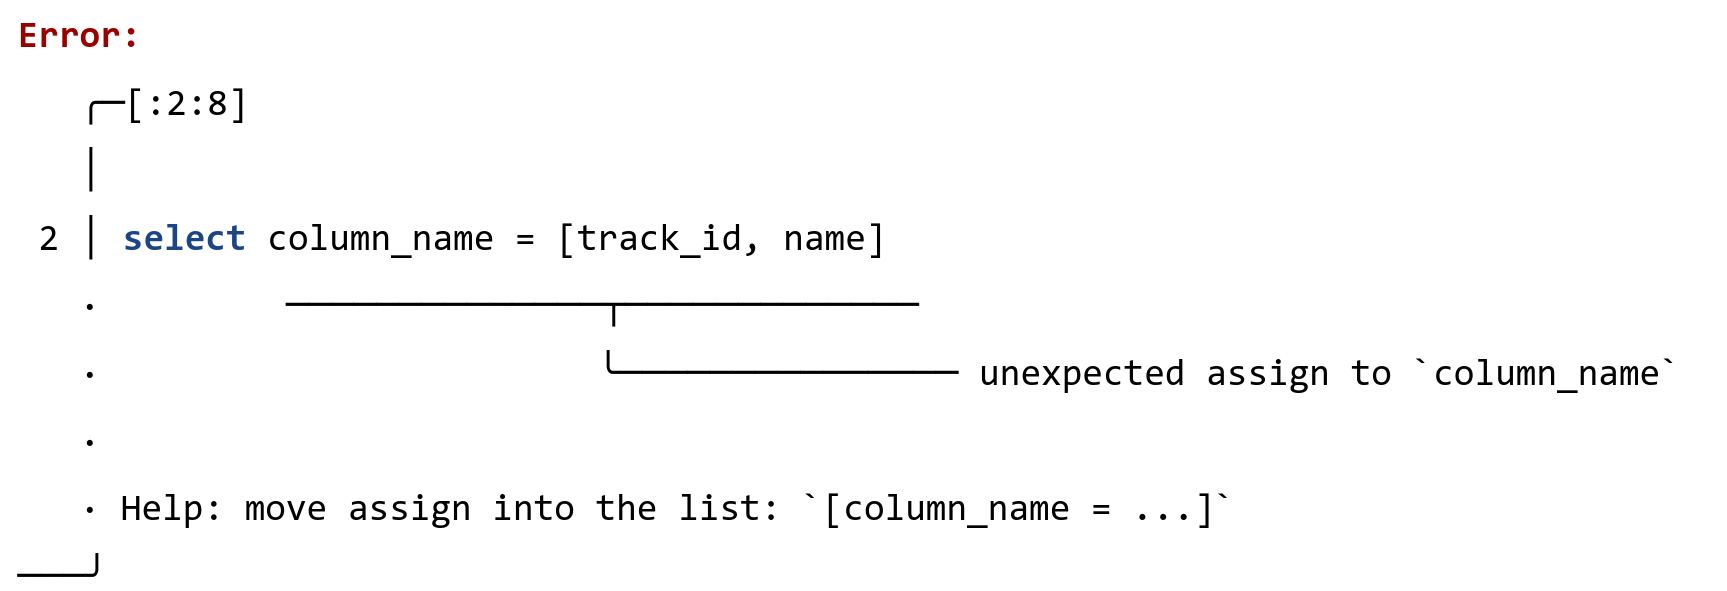
\includegraphics[width=0.9\textwidth]{images/error_message.png}
\vspace*{-3em}

\end{slide}

\begin{slide}{Architecture}

PRQL $\rightarrow$ PL $\rightarrow$ RQ $\rightarrow$ SQL

% TODO: example of PL and RQ  

\end{slide}

\begin{slide}{Licence}

% Language spec, docs, prqlc is open source

Apache

% all commits are on GH repo
% design is discussed in GH issues
% any PR is welcome 

Open community

% a language like this is hard to monetize
% even worse: affiliation with VC would have negative impact on adoption
% especially by opensource projects  
% thus: a slow but steady development pace

No plans to monetize

\end{slide}

\begin{slide}{Check it out: playground}
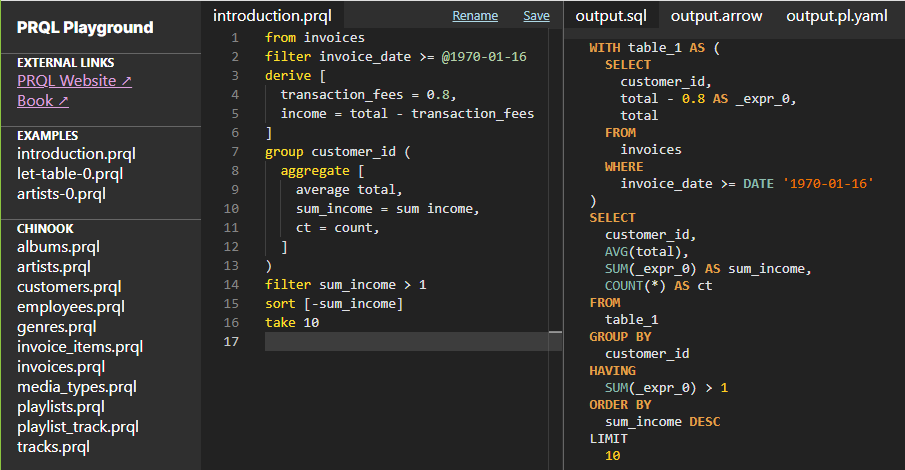
\includegraphics[width=0.8\textwidth]{images/playground.png}
\end{slide}

\begin{slide}{Check it out: VSCode extension}
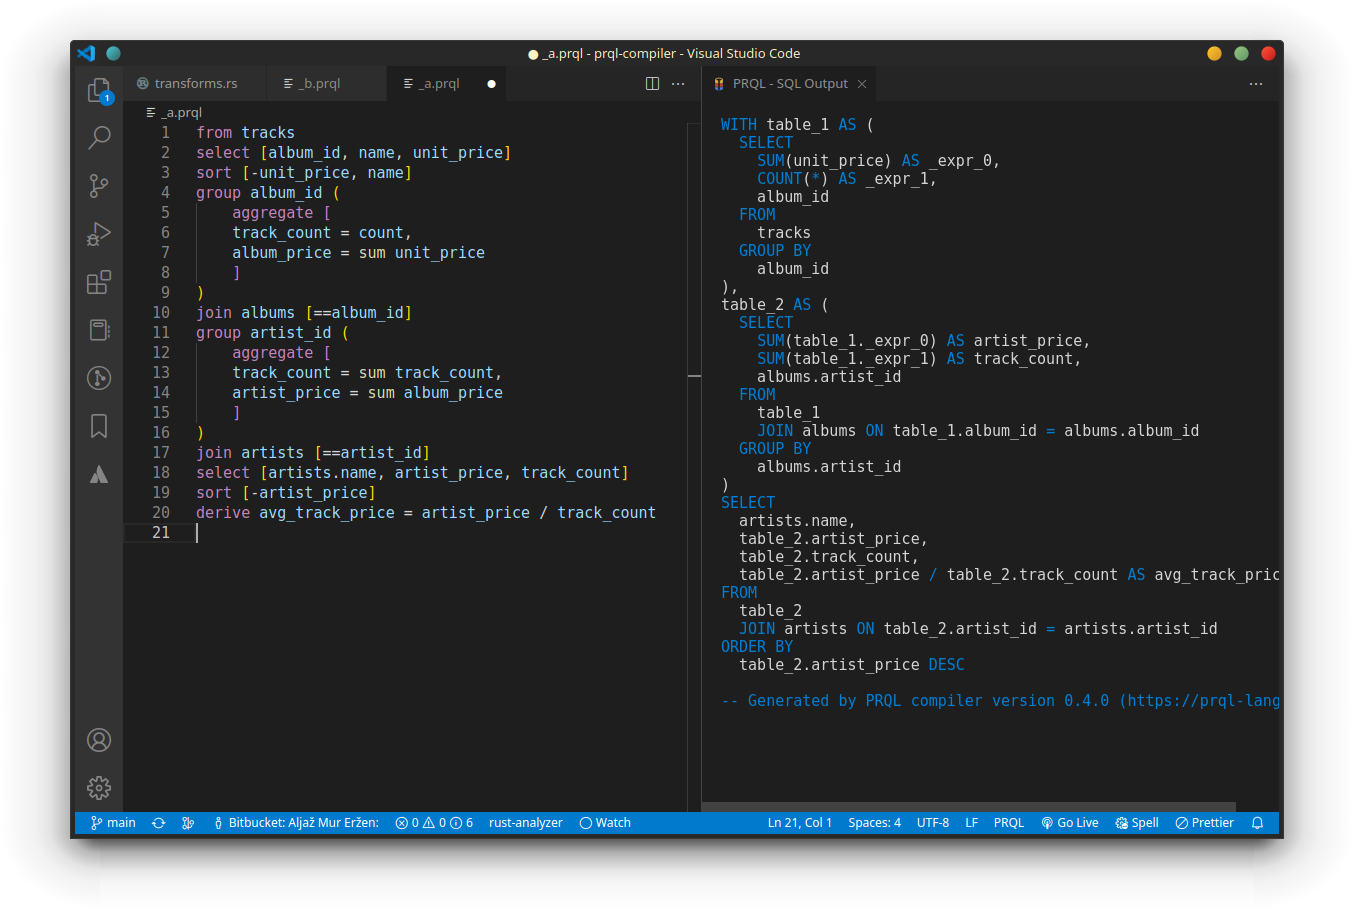
\includegraphics[width=0.7\textwidth]{images/vscode-ext.png}
\end{slide}

\begin{slide}{Check it out: prql-query - pq}
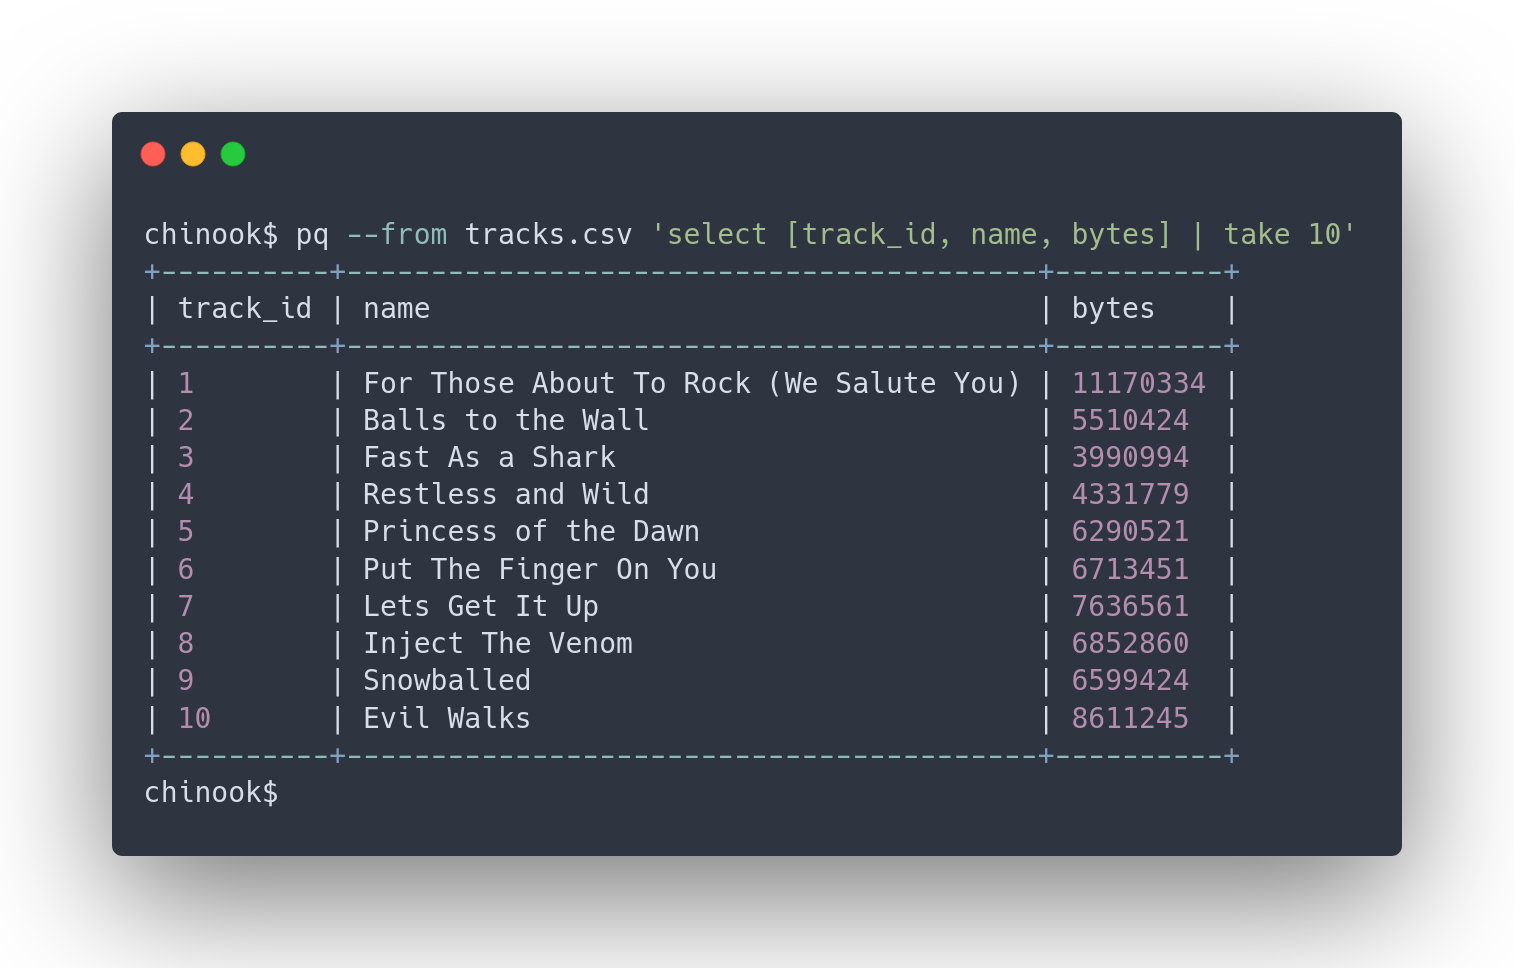
\includegraphics[width=0.7\textwidth]{images/pq.png}
\end{slide}

\begin{slide}{Check it out}

\begin{columns}
    \begin{column}{0.2\textwidth}
    \end{column}
    \begin{column}{0.5\textwidth}
        \begin{verbatim}
        pip install pyprql
        install.packages("prqlr")
        npm install prql
        cargo add prql-compiler
        \end{verbatim}
    \end{column}
\end{columns}

\vspace*{-2em}
\large

https://prql-lang.org

https://github.com/PRQL/prql

https://discord.gg/TfyM755m

\end{slide}

\end{document}
